\documentclass[border=10pt]{standalone}
\usepackage[svgnames]{xcolor}
\usepackage{amsmath}
\usepackage{pgfplots}
\pgfplotsset{compat=newest}
\usepackage[sfdefault]{FiraSans}
\usepackage{FiraMono}
\renewcommand*\familydefault{\sfdefault}
\begin{document}
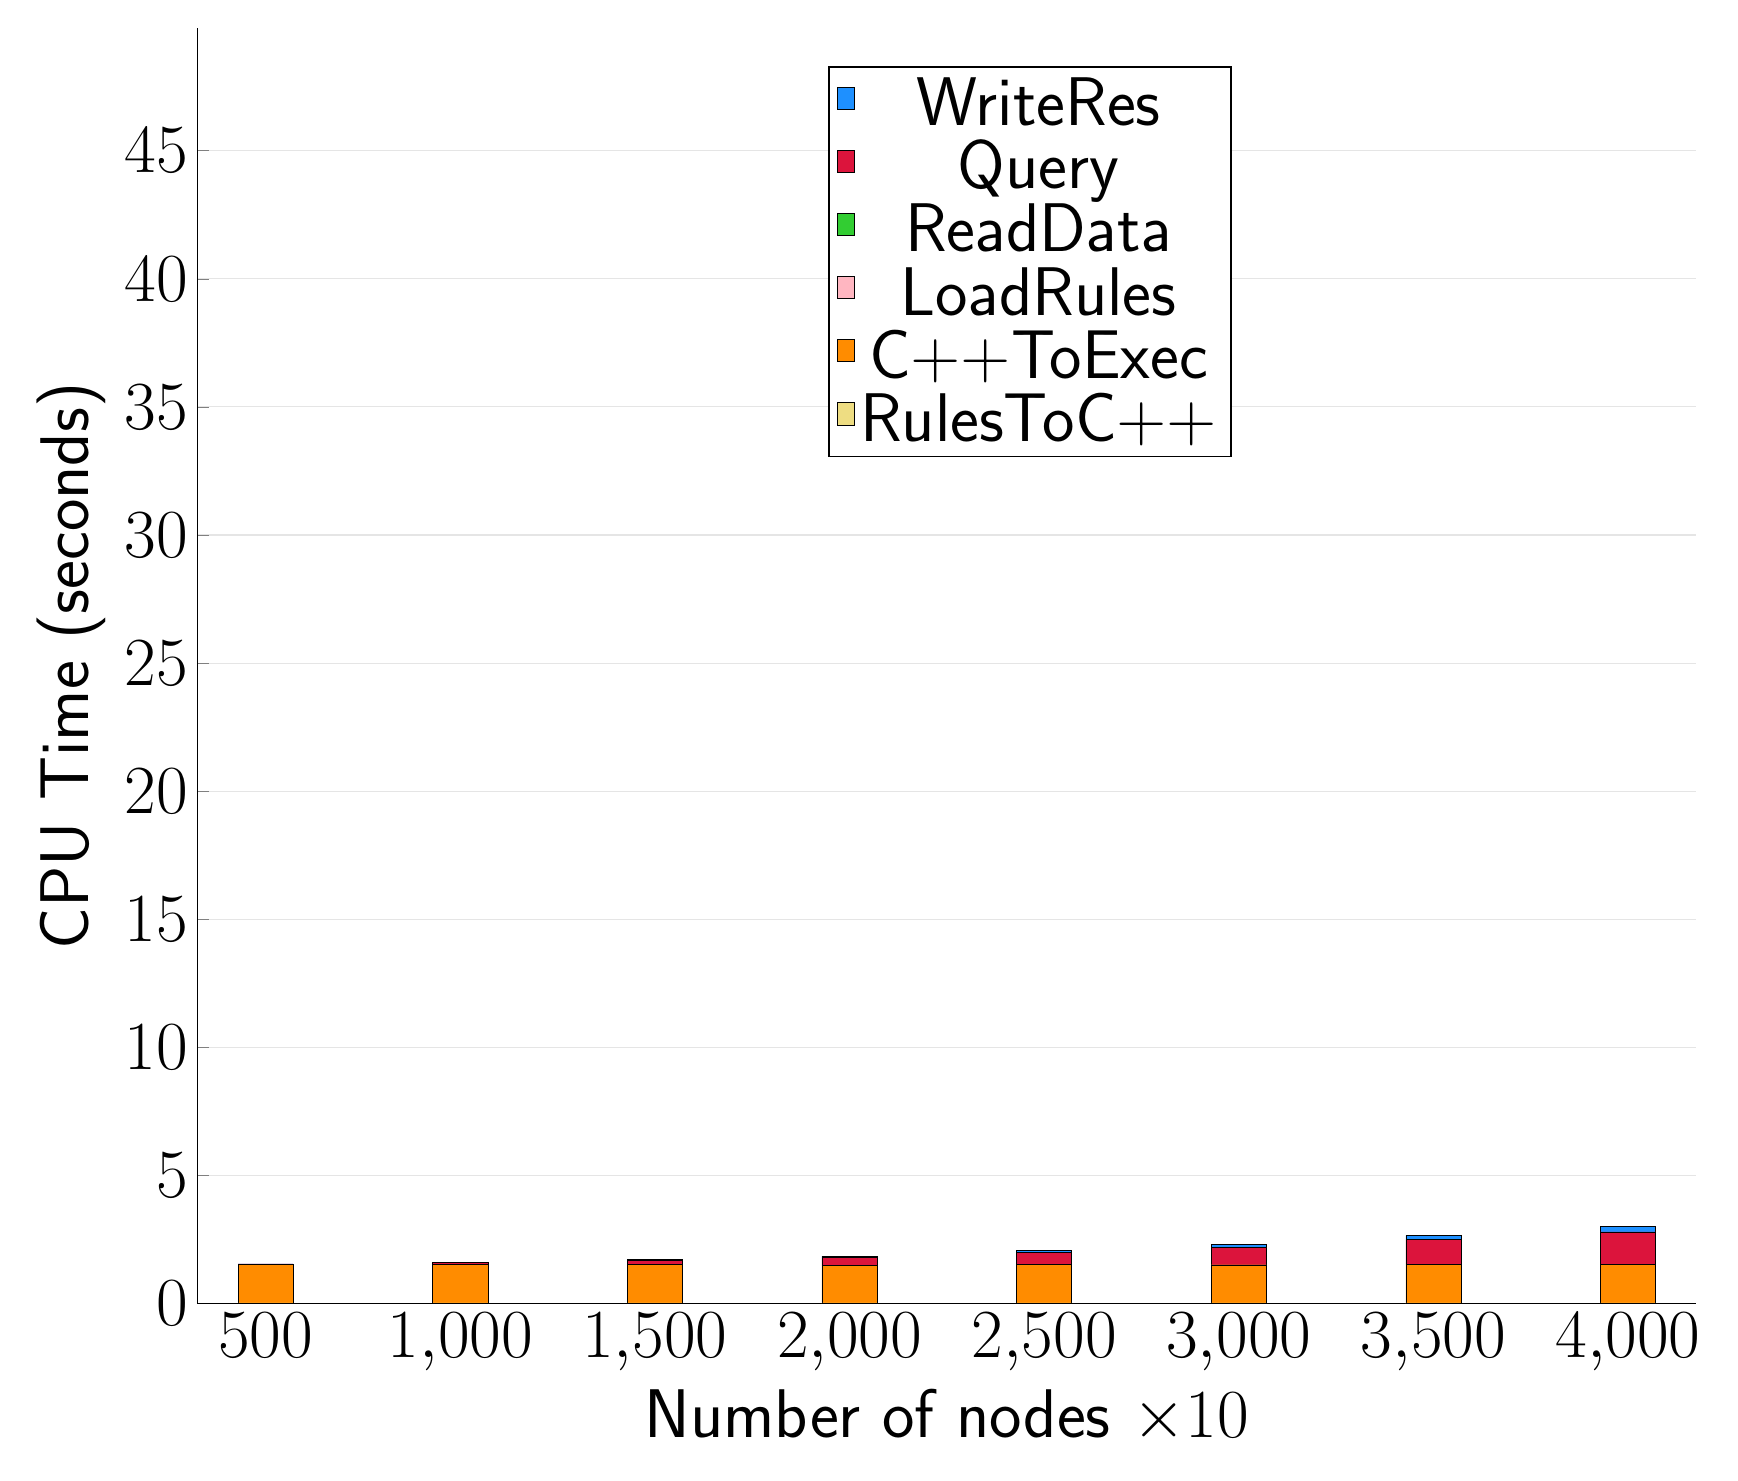
\begin{tikzpicture}
\begin{axis}[
   ybar stacked,
   width=1.7\textwidth,
   bar width=0.7cm,
   ymajorgrids, tick align=inside,
   major grid style={draw=gray!20},
   xtick=data,
   ymin=0, ymax=49.78293,
   axis x line*=bottom,
   axis y line*=left,
   enlarge x limits=0.05,
   legend style={
       at={(0.69, 0.97)},
       anchor=north east,
       legend columns=1,
       font=\Huge,
   },
   ylabel={CPU Time (seconds)},
   xlabel={Number of nodes $\times 10$},
   label style={font=\Huge},
   tick label style={font=\Huge},
]
\addlegendimage{fill=DodgerBlue, draw=black, line width=0.2pt}
\addlegendentry{WriteRes}
\addlegendimage{fill=Crimson, draw=black, line width=0.2pt}
\addlegendentry{Query}
\addlegendimage{fill=LimeGreen, draw=black, line width=0.2pt}
\addlegendentry{ReadData}
\addlegendimage{fill=LightPink, draw=black, line width=0.2pt}
\addlegendentry{LoadRules}
\addlegendimage{fill=DarkOrange, draw=black, line width=0.2pt}
\addlegendentry{C++ToExec}
\addlegendimage{fill=LightGoldenrod, draw=black, line width=0.2pt}
\addlegendentry{RulesToC++}
\addplot +[fill=LightGoldenrod, draw=black, line width=0.2pt] coordinates {
(500, 0.031000000000000007)
(1000, 0.030000000000000006)
(1500, 0.031000000000000007)
(2000, 0.030000000000000006)
(2500, 0.030000000000000006)
(3000, 0.030000000000000006)
(3500, 0.031000000000000007)
(4000, 0.03200000000000001)
};
\addplot +[fill=DarkOrange, draw=black, line width=0.2pt] coordinates {
(500, 1.496)
(1000, 1.495)
(1500, 1.4979999999999998)
(2000, 1.4700000000000002)
(2500, 1.497)
(3000, 1.4789999999999999)
(3500, 1.5050000000000001)
(4000, 1.504)
};
\addplot +[fill=LightPink, draw=black, line width=0.2pt] coordinates {
(500, 0.0)
(1000, 0.0)
(1500, 0.0)
(2000, 1.01e-05)
(2500, 0.0)
(3000, 0.0)
(3500, 0.0)
(4000, 0.0)
};
\addplot +[fill=LimeGreen, draw=black, line width=0.2pt] coordinates {
(500, 0.0011676)
(1000, 0.0022436)
(1500, 0.0032228)
(2000, 0.0043312)
(2500, 0.005075500000000001)
(3000, 0.006135099999999999)
(3500, 0.007208600000000001)
(4000, 0.008861399999999998)
};
\addplot +[fill=Crimson, draw=black, line width=0.2pt] coordinates {
(500, 0.0190286)
(1000, 0.0731685)
(1500, 0.160742)
(2000, 0.2923845)
(2500, 0.4639656)
(3000, 0.6832631000000001)
(3500, 0.9493334000000001)
(4000, 1.250394)
};
\addplot +[fill=DodgerBlue, draw=black, line width=0.2pt] coordinates {
(500, 0.004326100000000001)
(1000, 0.014152799999999998)
(1500, 0.0322575)
(2000, 0.056145)
(2500, 0.08829490000000001)
(3000, 0.1269263)
(3500, 0.1719552)
(4000, 0.2243158)
};
\end{axis}
\end{tikzpicture}

\end{document}
